\documentclass[border=6pt]{standalone}
\usepackage{amsmath}
\usepackage{tikz}
\usepackage{pgfplots}
\pgfplotsset{compat=1.18}
\usetikzlibrary{arrows.meta,calc,positioning}
\begin{document}
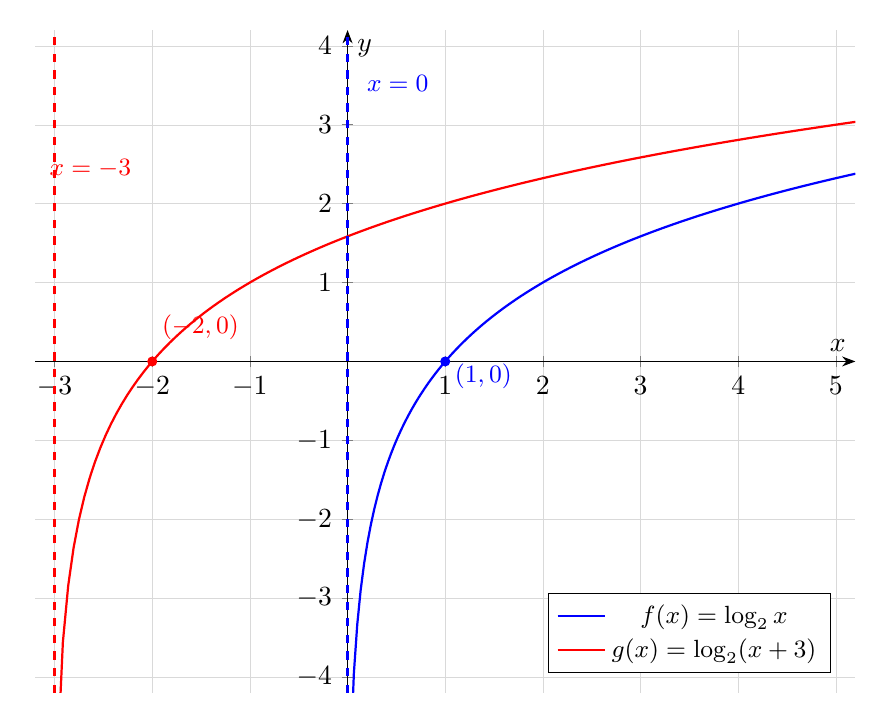
\begin{tikzpicture}
\begin{axis}[
    axis lines = middle,
    xlabel = {$x$}, ylabel = {$y$},
    xmin=-3.2, xmax=5.2, ymin=-4.2, ymax=4.2,
    xtick={-3,-2,-1,0,1,2,3,4,5},
    ytick={-4,-3,-2,-1,0,1,2,3,4},
    grid=both,
    grid style={line width=.1pt, draw=gray!30},
    width=12cm, height=10cm,
    axis line style={-Stealth},
    legend pos=south east,
    legend style={font=\small},
]
% parent f(x) = log2(x), domain x>0, vertical asymptote x=0
\addplot[domain=0.03:5.2, samples=150, thick, blue] {ln(x)/ln(2)};
\addlegendentry{$f(x)=\log_2 x$}

% translation g(x) = log2(x+3), domain x>-3, vertical asymptote x=-3
\addplot[domain=-2.97:5.2, samples=150, thick, red] {ln(x+3)/ln(2)};
\addlegendentry{$g(x)=\log_2(x+3)$}

% vertical asymptotes, dashed
\draw[dashed, blue, thick] (axis cs:0,-4.2) -- (axis cs:0,4.2);
\draw[dashed, red, thick] (axis cs:-3,-4.2) -- (axis cs:-3,4.2);

% x-intercepts
\addplot[only marks, mark=*, mark size=1.6pt, blue] coordinates {(1,0)};
\node[anchor=north west, blue] at (axis cs:1,0.1) {\small $(1,0)$};
\addplot[only marks, mark=*, mark size=1.6pt, red] coordinates {(-2,0)};
\node[anchor=south west, red] at (axis cs:-2,0.15) {\small $(-2,0)$};

\node[anchor=south west, blue] at (axis cs:0.1,3.3) {\small $x=0$};
\node[anchor=south west, red] at (axis cs:-3.15,2.2) {\small $x=-3$};

\end{axis}
\end{tikzpicture}
\end{document}
